\section{Travaux}
\subsection{Dummy}
\begin{frame}{Doctorat : multifractalité dans les quasicristaux}
\centering
Pavage quasipériodique :
~\\
~\\
\only<1>
{
\includegraphics[height=0.6\textheight]{img/1_travaux/no_overlap}

\phantom{presque périodique}

\phantom{Physique : alliages métalliques, atomes froids, bicouche de graphène}
}
\only<2>
{
\includegraphics[height=0.6\textheight]{img/1_travaux/overlap}

$\to$ presque périodes

Physique : alliages métalliques, atomes froids, bicouche de graphène
}
\end{frame}

\begin{frame}{Doctorat : multifractalité dans les quasicristaux}
\textbf{Motivation} : fonctions d'ondes \textbf{fractales}, physique \textbf{critique}

~

\begin{columns}
	\begin{column}{0.5\textwidth}
		1D : Chaîne de Fibonacci 
		
		{
		\centering
		\documentclass[../talk.tex]{subfiles}
\begin{document}


    	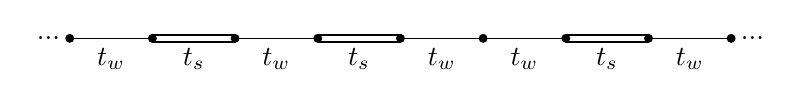
\begin{tikzpicture}[scale=.7]
    		\newcommand{\orig}{-1.5}
    		\newcommand{\trans}{1.5}
    		\newcommand{\vertspac}{-2.}
    		\newcommand{\vertsize}{0} % vertical span of the rectangles
    		\newcommand{\del}{.2}
    		\newcommand{\rad}{2pt} % radii of the circles

    		
    		% set the style of the strong bonds
    		\tikzset{
    			strong/.style={
    				double,
    				double distance=\rad,
    				line width=0.5pt
    				}
    		}
    	
    		% initial chain
    	
    		% bonds 
        	\draw[-] (\orig, 0)  node [left] {...}  -- (\orig+\trans, 0) node [midway, below] {$t_w$};
			\draw[strong] (\orig+\trans,0) -- (\orig+2*\trans,0) node [midway, below] {$t_s$};
			\draw[-] (\orig+2*\trans,0) -- (\orig+3*\trans,0) node [midway, below] {$t_w$};	
			\draw[strong] (\orig+3*\trans,0) -- (\orig+4*\trans,0) node [midway, below] {$t_s$};
			\draw[-] (\orig+4*\trans,0) -- (\orig+5*\trans,0) node [midway, below] {$t_w$};
			\draw[-] (\orig+5*\trans,0) -- (\orig+6*\trans,0) node [midway, below] {$t_w$};
			\draw[strong] (\orig+6*\trans,0) -- (\orig+7*\trans,0) node [midway, below] {$t_s$};
			\draw[-] (\orig+7*\trans,0) -- (\orig+8*\trans,0) node [right] {...} node [midway, below] {$t_w$};
    	
    		% sites
			\foreach \x in {0,...,8}
		      \filldraw (\orig+\x*\trans,0) circle (\rad); % node [below] {$\ket{\x}$};
		     
		    

		\end{tikzpicture}

\end{document}
		%
		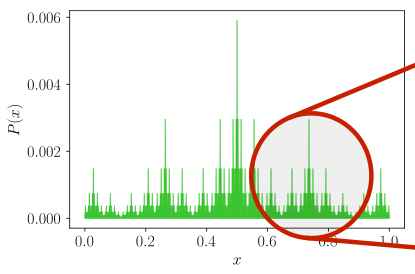
\includegraphics[width=\columnwidth]{img/1_travaux/heights}
		}
	\end{column}
	\begin{column}{0.5\textwidth}
		2D : Pavage octogonal
		\includegraphics[width=\columnwidth]{img/1_travaux/SKK}
	\end{column}
\end{columns}
\textbf{Méthodes} : groupe de renormalisation perturbatif, calcul variationnel (PRB 2016, 2017).
\end{frame}

\begin{frame}{Dimensions multifractales}
Dimensions fractales \textbf{exactes}, modèles \textbf{génériques} (PRB 2017)

\hfill {\footnotesize[Sutherland 86, Repetowicz \emph{et al} 98, Kalugin Katz 14]}

\begin{columns}
	\begin{column}{0.5\textwidth}
		\begin{align*}
			D_q(\lambda) &= \frac{q \theta(\lambda) - \theta(\lambda^q))}{(q-1)\theta(1)} \\
			\theta_{1D}(\lambda) &= \arcsin\left(\frac{(\lambda + \lambda^{-1})^2}{2}\right) \\
			\theta_{2D}(\lambda) &= \arccos(4\lambda + 9 + 4\lambda^{-1})
		\end{align*}
	\end{column}
	\begin{column}{0.5\textwidth}
		Transport \textbf{anormal}
		\centering
		\includegraphics[width=0.9\columnwidth]{img/1_travaux/transport}
	\end{column}
\end{columns}

\textbf{Perspectives} : topologie, robustesse (désordre, interactions).
\end{frame}

\begin{frame}{Postdoc : interactions, localisation à $N$ corps}
\begin{block}{\textbf{Dynamique quantique}, en présence d'\textbf{interactions fortes} et de \textbf{désordre}}
	\begin{enumerate}
		\item Générique :  \textcolor{comp}{thermalisation, décohérence rapide},
		\item Inhabituel : \textcolor{BostonBlue}{non-ergodicité, cohérence longue, \textbf{localisation à $N$ corps}}.
	\end{enumerate}
\end{block}

\begin{columns}
\begin{column}{0.5\textwidth}
\centering
\includegraphics[width=0.9\columnwidth]{img/1_travaux/Imbalance_Choi_thermal}

\includegraphics[width=0.9\columnwidth]{img/1_travaux/Imbalance_Choi}

[Choi \emph{et al} 16]
\end{column}
\begin{column}{0.5\textwidth}
\textbf{Expériences} : atomes/ions froids. Films supraconducteurs ?

\textbf{Motivations} : transition de phase thermal-localisé, nature phase localisée

\textbf{Méthodes} : diagonalisation exacte

taille record $L=26$ (SciPost 2018)
\end{column}
\end{columns}
\end{frame}

\begin{frame}{Postdoc : un modèle de la localisation à $N$ corps}
Fermions en interaction :
\[
	H = \sum_{i=1}^L \left[ J (c_i^\dagger c_{i+1} + \text{h.c}) + \Delta n_i n_{i+1} - h_i n_i \right]
\]

{
\centering
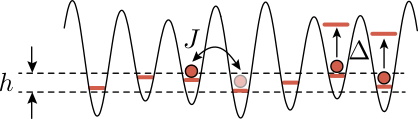
\includegraphics[width=0.5\textwidth]{img/1_travaux/XXZ_cold_atoms}

}
Modèle générique : décrit fermions, spins, bosons de cœur dur.

Désordre : pilote la transition de phase :

{
\centering
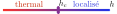
\includegraphics[width=0.5\textwidth]{img/1_travaux/arrow}

}
\end{frame}

\begin{frame}{Postdoc : localisation à $N$ corps \& multifractalité}
\begin{columns}
	\begin{column}{0.5\textwidth}
		États propres dans la phase localisée ?
	
		\textbf{Multifractalité} dans l'espace de Hilbert (arxiv 2018)
		
		Espace de Hilbert : graphe complexe, $\text{Vol} \sim 2^L/\sqrt{L}$
		
		\centering		
		\includegraphics[width=0.6\columnwidth]{img/1_travaux/graph_L_6}
	\end{column}
	\begin{column}{0.5\textwidth}
		{		
		\centering
		\includegraphics[width=0.8\columnwidth]{img/1_travaux/scalings}
		
		}		
		Analyse d'échelle : sonde les phases thermales et localisées et leur transition
				
	\end{column}
\end{columns}
\textbf{Perspectives} : nature phase thermale, localisation en 2D, conditions non-thermalisation
\end{frame}